\subsection{RAID Structure}\label{subsec:RAID_Structure}
Having a large number of disks in a system presents opportunities for improving the rate at which data can be read or written, if the disks are operated in parallel.
It also offers the potential for improving the reliability of data storage, because redundant information can be stored on multiple disks.
Allowing the failure of one disk to prevent loss of data.

\begin{definition}[RAID]\label{def:RAID}
  \emph{RAID} (\emph{Redundant Array of Independent Disks}) is a collection of disk-organization techniques.
  These allow multiple physically separate disks to be viewed by the \nameref{def:Operating_System} as a single, larger, logical disk.

  There are 2 main ways to implement support for RAID:\@
  \begin{enumerate}[noitemsep]
  \item \textbf{Software RAID}.
    This relies on the \nameref{def:Kernel} and \nameref{def:Operating_System} handling the disks for RAID functionality.
    This means that the RAID-ed disks cannot be used for booting, because the RAID modules are only loaded once the kernel is loaded.

  \item \textbf{Hardware RAID}.
    There are 2 alternatives here.
    \begin{enumerate}[noitemsep]
    \item RAID support is built into the hardware.
    \item RAID support is not built into the hardware, and a separate RAID card must be used.
    \end{enumerate}
  \end{enumerate}

  There are a variety of levels to RAID, each of which has different properties.
\end{definition}

\subsubsection{Reliability via Redundancy}\label{subsubsec:RAID_Reliability_Redundancy}
If we store extra information that is not normally needed but that can be used in the event of failure of a disk to rebuild the lost information, we can greatly improve reliability.
Thus, even if a disk fails, data are not lost.

The simplest and most expensive approach to introducing redundancy is to duplicate the contents of every disk onto another.
This technique is called mirroring.
With mirroring, a logical volume consists of two physical disks, and every write is carried out on both disks simultaneously.
The result is called a mirrored \nameref{def:Volume}.
Data will be lost only if the second disk fails before the first failed disk is replaced.

However, power failures are a particular source of concern, since they occur far more frequently than natural disasters.
Even with mirroring of disks, if writes are in progress to the same block in both disks, and power fails before both blocks are fully written, the two blocks can be in an inconsistent state.
The usual solution is to add a write-cache, typically called solid-state nonvolatile RAM (NVRAM) to the RAID array.
This write-back cache is protected from data loss during power failures, so the write can be considered complete when it is written to the cache, since even if there is a failure, no data is lost.

\subsubsection{Performance via Parallelism}\label{subsubsec:RAID_Performance_Parallelism}
With disk mirroring, the rate at which \textbf{read} requests can be handled is doubled, since read requests can be sent to either disk (as long as both disks in a pair are functional).
The \textbf{transfer} and \textbf{write} rate of each read is the same as in a single-disk system.

With multiple disks, we can improve the transfer rate by striping data across the disks.
Data striping consists of splitting a unit of data across multiple disks.
However, this also means that if any single disk were to fail, all data would be unrecoverable.

There are several types of striping that is possible:
\begin{itemize}[noitemsep]
\item Bit-level Striping, where each bit of every byte is striped across the disks.
\item Block-level striping, where blocks of a \nameref{def:File} are striped across the disks.
\item Sector-level striping.
\item etc.
\end{itemize}

The main goals of using striping in the parallel manner are:
\begin{enumerate}[noitemsep]
\item Increase the throughput of multiple small accesses (page accesses) by load balancing.
\item Reduce the response time of large accesses.
\end{enumerate}

\subsubsection{RAID Levels}\label{subsubsec:RAID_Levels}
Numerous schemes to provide redundancy at lower cost by using disk striping combined with ``parity'' bits have been proposed.
These schemes have different cost–performance trade-offs and are classified according to RAID levels.

$P$ indicate error-correcting bits and $C$ indicates a copy of the data.
\begin{figure}[h!tbp]
  \centering
  \begin{subfigure}{1.0\linewidth}
    \centering
    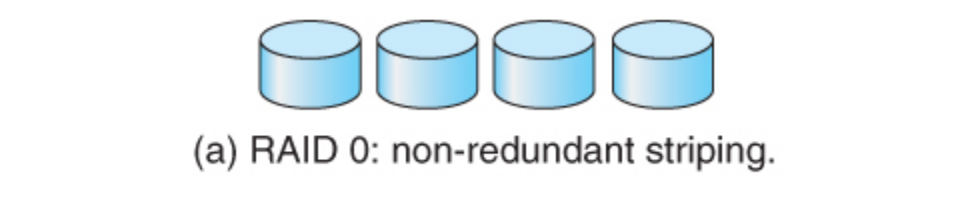
\includegraphics[scale=1.00]{./Drawings/EDAF35-Operating_Systems/RAID_0.png}
    \caption{\nameref{par:RAID_0}: Striped Disks}
    \label{subfig:RAID_0}
  \end{subfigure} \\
  \begin{subfigure}{0.45\linewidth}
    \centering
    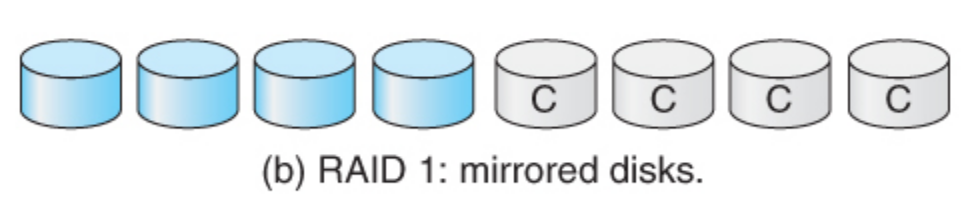
\includegraphics[scale=1.00]{./Drawings/EDAF35-Operating_Systems/RAID_1.png}
    \caption{\nameref{par:RAID_1}: Mirrored Disks}
    \label{subfig:RAID_1}
  \end{subfigure}
  \begin{subfigure}{0.45\linewidth}
    \centering
    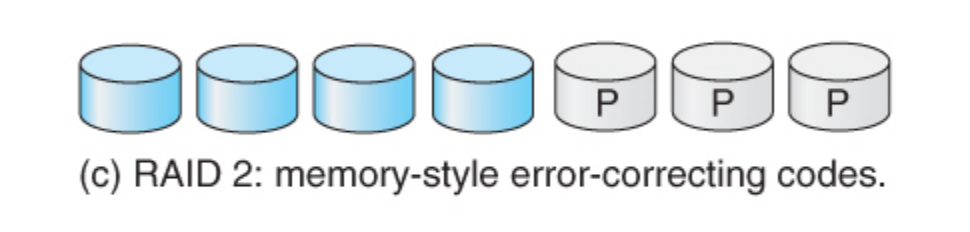
\includegraphics[scale=1.00]{./Drawings/EDAF35-Operating_Systems/RAID_2.png}
    \caption{\nameref{par:RAID_2}: ECC Disks}
    \label{subfig:RAID_2}
  \end{subfigure} \\
  \begin{subfigure}{0.45\linewidth}
    \centering
    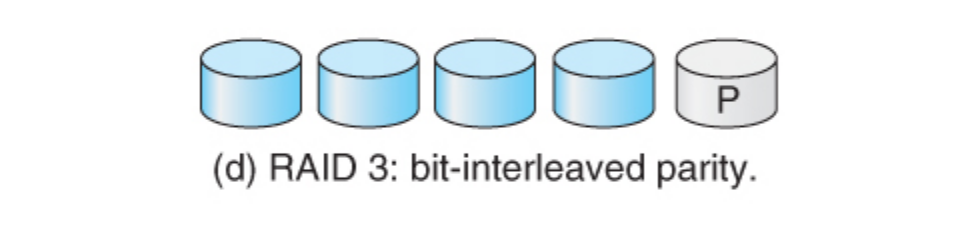
\includegraphics[scale=1.00]{./Drawings/EDAF35-Operating_Systems/RAID_3.png}
    \caption{\nameref{par:RAID_3}: Bit-Interleaved Parity}
    \label{subfig:RAID_3}
  \end{subfigure}
  \begin{subfigure}{0.45\linewidth}
    \centering
    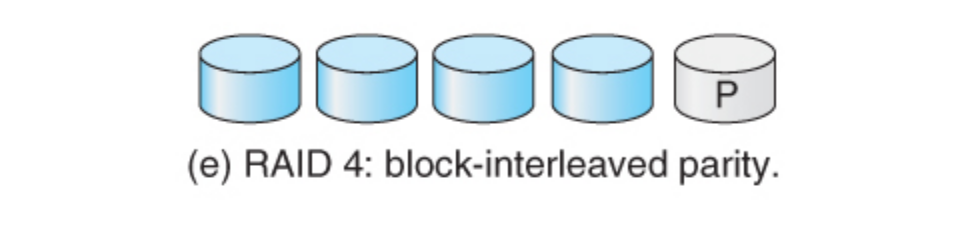
\includegraphics[scale=1.00]{./Drawings/EDAF35-Operating_Systems/RAID_4.png}
    \caption{\nameref{par:RAID_4}: Block-Interleaved Parity}
    \label{subfig:RAID_4}
  \end{subfigure} \\
  \begin{subfigure}{0.45\linewidth}
    \centering
    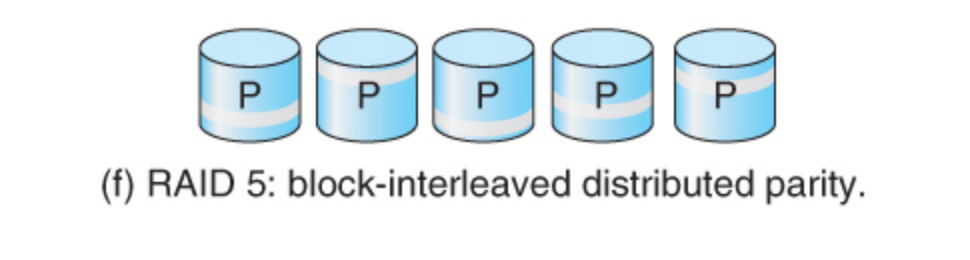
\includegraphics[scale=1.00]{./Drawings/EDAF35-Operating_Systems/RAID_5.png}
    \caption{\nameref{par:RAID_5}: Block-Interleaved $P$ Parity}
    \label{subfig:RAID_5}
  \end{subfigure}
  \begin{subfigure}{0.45\linewidth}
    \centering
    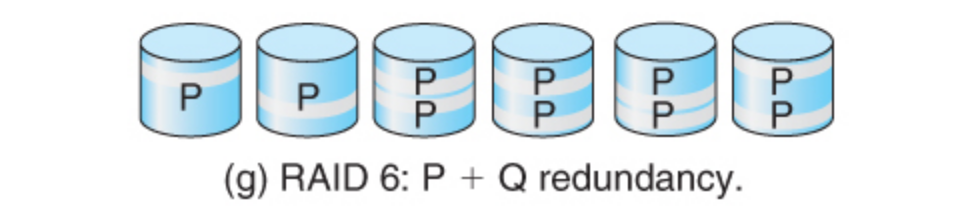
\includegraphics[scale=1.00]{./Drawings/EDAF35-Operating_Systems/RAID_6.png}
    \caption{\nameref{par:RAID_6}: Block-Interleaved $P+Q$ Parity}
    \label{subfig:RAID_6}
  \end{subfigure} \\
  \begin{subfigure}{0.45\linewidth}
    \centering
    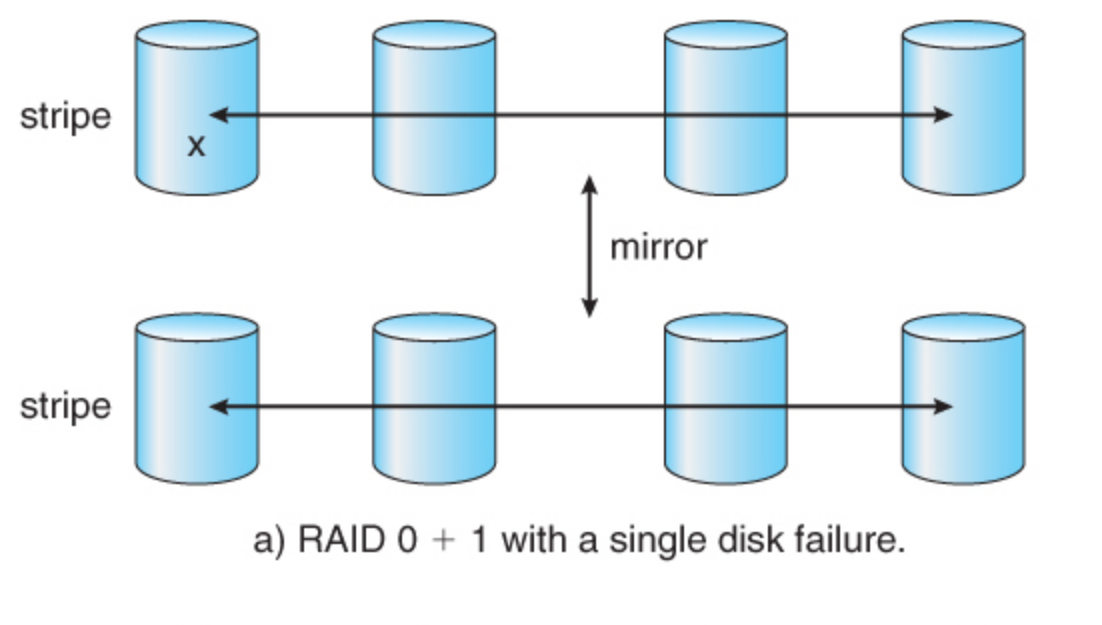
\includegraphics[scale=1.00]{./Drawings/EDAF35-Operating_Systems/RAID_01.png}
    \caption{\nameref{par:RAID_01}: Mirrored Stripes}
    \label{subfig:RAID_01}
  \end{subfigure}
  \begin{subfigure}{0.45\linewidth}
    \centering
    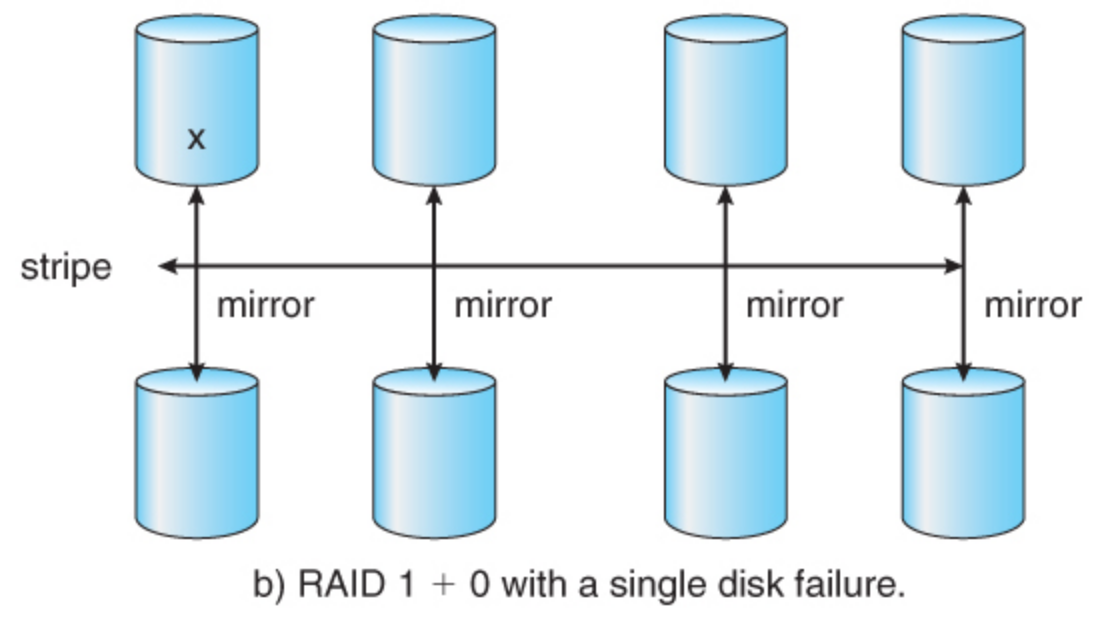
\includegraphics[scale=1.00]{./Drawings/EDAF35-Operating_Systems/RAID_10.png}
    \caption{\nameref{par:RAID_10}: Striped Mirrors}
    \label{subfig:RAID_10}
  \end{subfigure} \\
  \caption{RAID Levels}
  \label{fig:RAID_Levels}
\end{figure}

\paragraph{RAID 0}\label{par:RAID_0}
RAID level 0 refers to disk arrays with block striping without any redundancy.

Seen in \Cref{subfig:RAID_0}.

\paragraph{RAID 1}\label{par:RAID_1}
RAID level 1 refers to full-disk mirroring.

\Cref{subfig:RAID_1} shows a mirrored organization.

\paragraph{RAID 2}\label{par:RAID_2}
RAID level 2 is also known as memory-style error-correcting-code (ECC) organization.
Each byte in a memory system may have a parity bit associated with it that records whether the number of bits in the byte set to 1 is even (parity = 0) or odd (parity = 1).
If one of the bits in the byte is damaged (including the stored parity bit), the parity of the entire byte changes and thus does not match the stored parity.
Thus, all single-bit errors are detected by the memory system.
Error-correcting schemes store two or more extra bits and can reconstruct the data if any single bit is damaged.
If one of the disks fails, the remaining bits of the byte and the associated error-correction bits can be read from other disks and used to reconstruct the damaged data.

Seen in \Cref{subfig:RAID_2}.

\paragraph{RAID 3}\label{par:RAID_3}
RAID level 3, improves on \nameref{par:RAID_2} by taking into account that disk controllers can detect whether a sector has been read correctly, so a single parity bit can be used for error correction as well as for detection.
RAID level 3 has two advantages over level 1.
\begin{enumerate}[noitemsep]
\item The storage overhead is reduced because only one parity disk is needed for several regular
disks.
\item Reads/writes of a byte are spread out over multiple disks with $N$-way striping of data, the transfer rate for reading or writing a single block is $N$ times as fast as with \nameref{par:RAID_1}.
\end{enumerate}

On the negative side:
\begin{enumerate}[noitemsep]
\item RAID level 3 supports fewer I/Os per second, since every disk has to participate in every I/O request.
\item The expense of computing and writing the parity is not minor.
\end{enumerate}

Seen in \Cref{subfig:RAID_3}.

\paragraph{RAID 4}\label{par:RAID_4}
RAID level 4 uses block-level striping, as in \nameref{par:RAID_0} and keeps a parity block on a separate dedicated disk for corresponding blocks from $N$ other disks.
If one of the disks fails, the parity block can be used with the corresponding blocks from the other disks to restore the blocks of the failed disk.

A block read accesses only one disk, allowing other requests to be processed by the other disks.
Thus, the data-transfer rate for each access is slower, but a higher overall I/O rate.
The transfer rates for large reads are high, since multiple read accesses can proceed in parallel.
Large writes also have high transfer rates, since the data and parity can be written in parallel.
Small independent writes cannot be performed in parallel.

Seen in \Cref{subfig:RAID_4}.

\paragraph{RAID 5}\label{par:RAID_5}
RAID level 5, or block-interleaved distributed parity, differs from \nameref{par:RAID_4} in that it spreads data and parity among all $N + 1$ disks.
For each block, one of the disks stores the parity and the others store data.
A parity block cannot store parity for blocks in the same disk, because a disk failure would result in loss of data as well as of parity, making the loss recoverable.
By spreading the parity across all the disks in the set, RAID 5 avoids potential overuse of a single parity disk, which can occur with RAID 4.

The data for the $n$th block in an array with $D$ disks is stored on disk $(n \bmod D) + 1$.

Seen in \Cref{subfig:RAID_5}.

\paragraph{RAID 6}\label{par:RAID_6}
RAID level 6 is similar to \nameref{par:RAID_5} but stores more redundant information to guard against multiple disk failures.
Instead of parity, error-correcting codes are used.
2 bits of redundant data are stored for every 4 bits of data allowing the system to tolerate two disk failures.

Seen in \Cref{subfig:RAID_6}.

\paragraph{RAID 01}\label{par:RAID_01}
RAID 01 (read RAID zero-one) refers to a combination of \nameref{par:RAID_0} and \nameref{par:RAID_1}.
RAID 0 provides the performance, while RAID 1 provides the reliability.
Generally, this level provides better performance than \nameref{par:RAID_5}.
Unfortunately, it doubles the number of disks needed for storage, so it is also relatively expensive.
A set of disks are striped, and then the stripe is mirrored to another, equivalent stripe.

Seen in \Cref{subfig:RAID_01}.

\paragraph{RAID 10}\label{par:RAID_10}
RAID 10 (read RAID one-zero), mirrors disks into pairs, then the resulting mirrored pairs are striped.

Seen in \Cref{subfig:RAID_10}.

\subsubsection{Choosing a RAID Level}\label{subsubsec:Choosing_RAID_Level}
Some considerations are:
\begin{itemize}[noitemsep]
\item Rebuild performance.
  If a disk fails, the time needed to rebuild its data can be significant.
  This may be an important factor if a continuous supply of data is required.
  Furthermore, rebuild performance influences the mean time to failure.
  RAID system designers and administrators of storage have to make several other decisions as well.

\item The number of disks in a given RAID set.

\item The number of bits that are protected by each parity bit.
  If more disks are in an array, data-transfer rates are higher, but the system is more expensive.
  If more bits are protected by a parity bit, the space overhead due to parity bits is lower, but the chance that a second disk will fail before the first failed disk is repaired is greater, and that will result in data loss.
\end{itemize}

%%% Local Variables:
%%% mode: latex
%%% TeX-master: "../../EDAF35-Operating_Systems-Reference_Sheet"
%%% End:
